\documentclass[11pt,a4paper]{article}
\usepackage{ucs}
\usepackage[T1]{fontenc}
\usepackage[utf8x]{inputenc}
\usepackage[english]{babel}
\usepackage{amsmath}
\usepackage{amsfonts}
\usepackage{amssymb}
\usepackage{graphicx}
\usepackage{shadethm}
\usepackage{caption}
\usepackage{tikz} 
\usepackage{geometry}
\usepackage{longtable}
\usepackage{units}
\usepackage{float}
\usepackage{braket}
\usepackage{subfigure}


\geometry{
    left=2cm,
    right=2cm,
    top=2cm,
    bottom=2.8cm,
    bindingoffset=5mm
}

\newcommand{\minipanf}{\begin{minipage}{\linewidth}}
\newcommand{\minipend}{\end{minipage}}
\newcommand{\abs}[1]{\ensuremath{\left\vert#1\right\vert}}

\begin{document}

\begin{titlepage}
\newcommand{\HRule}{\rule{\linewidth}{0.5mm}} % Defines a new command for the horizontal lines, change thickness here

\center % Center everything on the page
 
%----------------------------------------------------------------------------------------
%	HEADING SECTIONS
%----------------------------------------------------------------------------------------

\textsc{\LARGE TU Dresden}\\[1.5cm] % Name of your university/college
\textsc{\Large Advanced practical course}\\[0.5cm] % Major heading such as course name
\textsc{\Large Lab report}\\[0.5cm] % Major heading such as course name

%----------------------------------------------------------------------------------------
%	TITLE SECTION
%----------------------------------------------------------------------------------------

\HRule \\[0.7cm]
{ \huge \bfseries Nuclear Magnetic Resonace}\\[0.4cm] % Title of your document
\HRule \\[1.5cm]
 
%----------------------------------------------------------------------------------------
%	AUTHOR SECTION
%----------------------------------------------------------------------------------------

\begin{minipage}{0.4\textwidth}
\begin{flushleft} \large
\emph{Authors:}\\
Toni \textsc{Ehmcke}\\
Christian \textsc{Siegel}
\end{flushleft}
\end{minipage}
~
\begin{minipage}{0.4\textwidth}
\begin{flushright} \large
\emph{Supervisor:} \\
Rajib \textsc{Sarkar} % Supervisor's Name
\end{flushright}
\end{minipage}\\[4cm]

%----------------------------------------------------------------------------------------
%	DATE SECTION  
%----------------------------------------------------------------------------------------

{\large Dresden,\selectlanguage{english} \today}\\ % Date, change the \today to a set date if you want to be precise
{\large Date of experimental procedure: November 19th, 2015}\\[3cm]


\vfill 

\end{titlepage} 	% Titelseite

\tableofcontents
\newpage 

\section{Introduction}
	\subsection{Motivation}
		\textit{Nuclear Magnetic Resonance} is a physical phenomenon that can be observed while placing an ensemble of nuclei into a static magnetic field and stimulate it with a high-frequent alterning field. A necessary condition for this effect is that the atoms of the sample have a \textit{nuclear spin} different from zero. It is the central concept that is used for \textit{NMR-Spectroscopy}, a standard methodology for the investigation of the structure and interaction of complex molecules and solid state bodies by measuring local magnetic fields, and the \textit{magnetic resonance tomography} which is an imaging technique used in clinical diagnistics for describing the morphilogic and physiologic build-up of tissues and organs. For all of those applications we need to find out some central parameters of particular physical compensation-processes, the so called \textit{relaxation times} $T_1$ and $T_2$. In the following experiment exactly those material-characteristic obserables are determined for an ensemble of $^57$Fe-nuclei. But at first some basic knowledge.
	\subsection{Nuclear Zeeman-Effect}		% introduction: physical basics + task
\section{Experimental procedure}

    The followoing task had to be done:\\
    \textbf{\ref{task_1}}: Preparation of a radio frequency resonant circuit with the insertion of an iron powde probe in a cryostate\\
    \textbf{\ref{task_2}}: Find the nuclear spin resonance by varying the NMR-pulse frequency while recording a spectrum of the $^{57}$Fe nuclear spin ensemble and calculation of the local magnetic field\\
    \textbf{\ref{task_3}}: Optimization of the pulse sequence by recording a rotation angle curve\\
    \textbf{\ref{task_4}}: Find the spin-spin- and spin-lattice relaxation constants $T_2 \text{ and } T_1$.   

	\subsection{Preparation of a high frequency resonant circuit}
    \label{task_1}
    First one has to prepare a copper coil with a diameter big enough to hold an iron powder assay. After the coil is wrapped one has to sold it onto the contacts of a stick, which provides a mechanism to tune the measured frequency to find the resonance frequency. While solding one has to be careful to make sure, that one do not take to much tin, because the resisteaces of tin and copper are different. In the same way the soldered point should connect the contact and the coil directly, otherwise this could influence the results while tuning to the resonance frequency.
    \begin{center}
           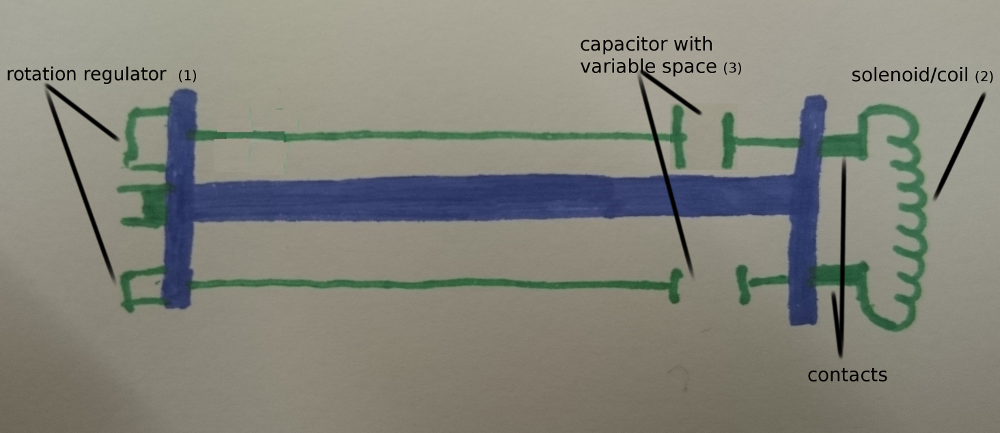
\includegraphics[scale=0.4]{pic/Skizze_Sonde.png} 
           \captionof{figure}{basic sketch of a probe with a coil on it}
           \label{fig:sketch}
    \end{center}
    The rotation regulator (\ref{fig:sketch}.1) varies the space between the capacitor's plates (\ref{fig:sketch}.3) so one can tune the frequency of the solenoid (\ref{fig:sketch}.2).
    \subsection{Finding of the nuclear spin resonance by varying the pulse frequency}
    \label{task_2}
    After the preparation of the solenoid and the insertion of the probe into the cryostat one has to mention what the different paramters built in the measurement-software do with the curves. The different parameters one could vary are $pw$, $\tau$, $rd$ and $ad$. $pw$ makes the magnitude look more gaussian and gives it a bigger value by make the imaginary and real parts more oscillating the higher it is. Varying $\tau$ shows less oscillations and a lower magnitude the higher $\tau$ is. At least one can also vary the parameter $rd$. The higher it is, the more oscillations can be found. These parameters are choosed such that the magnitude fits better to a gaussian. This means, one searches parameters with a low amount of oscillations, which also have not a big intensity. After the best parameters ($ pw=2\unit{\mu s},\ \tau = 60\unit{\mu s},\ rd = 15\unit{\mu s},\ ad=10\unit{\mu s} $) are found, one looks  at the behavior of the curve at the resonance frequency, a little bit below and a bit above as shown in the figures \ref{beltd} - \ref{abofs}.\\
        \begin{figure}[H]
            \subfigure[intensity below resonance frequency in time domain\label{beltd}]{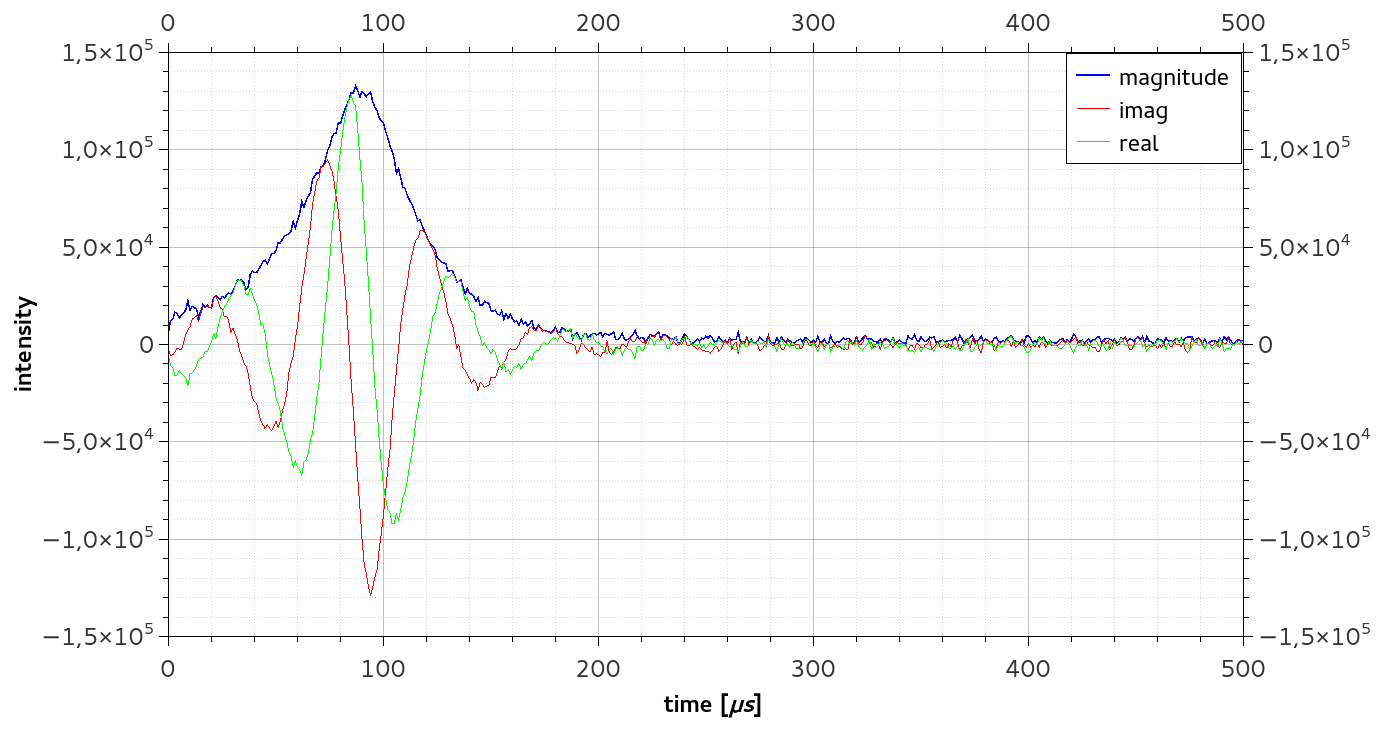
\includegraphics[scale=0.225]{pic/below_resfreq_td.png}}
            \subfigure[intensity below resonance frequency in fourier space\label{belfs}]{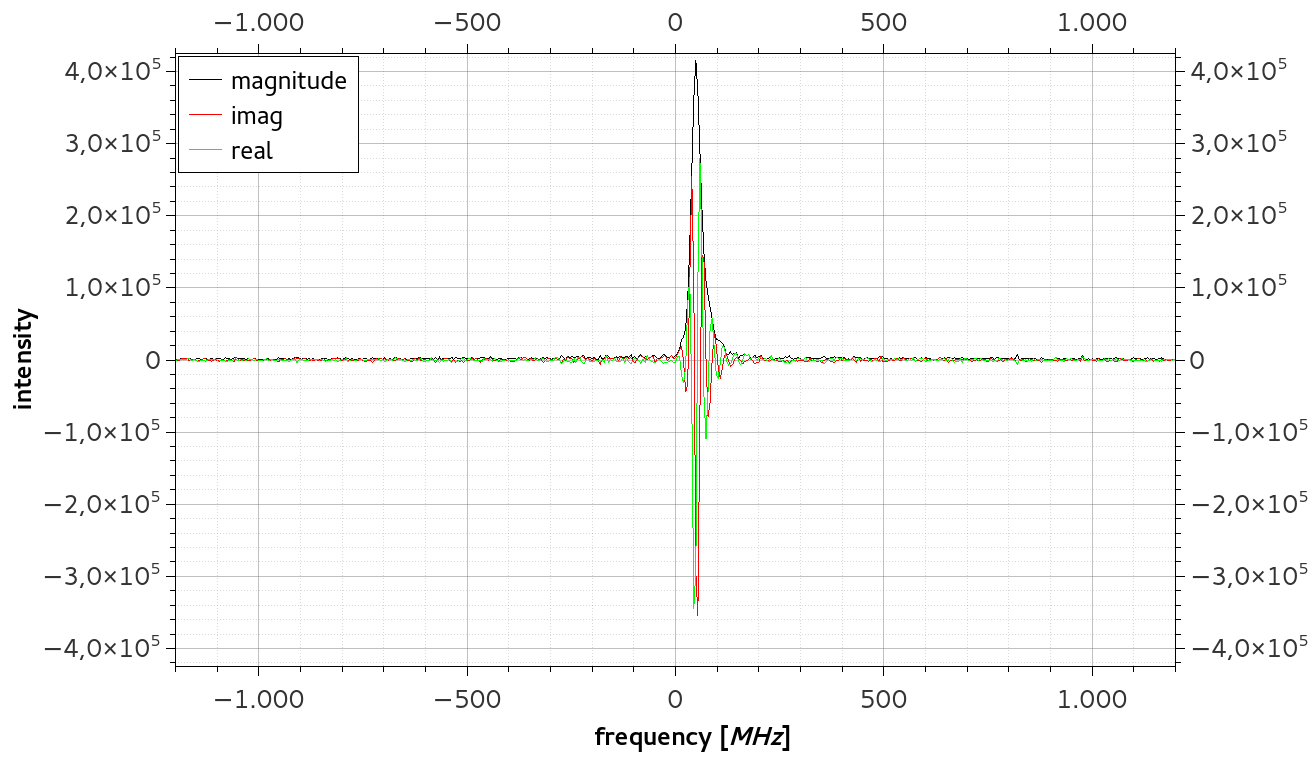
\includegraphics[scale=0.225]{pic/below_resfreq_fs.png}}
            \subfigure[intensity at resonance frequency in time domain\label{restd}]{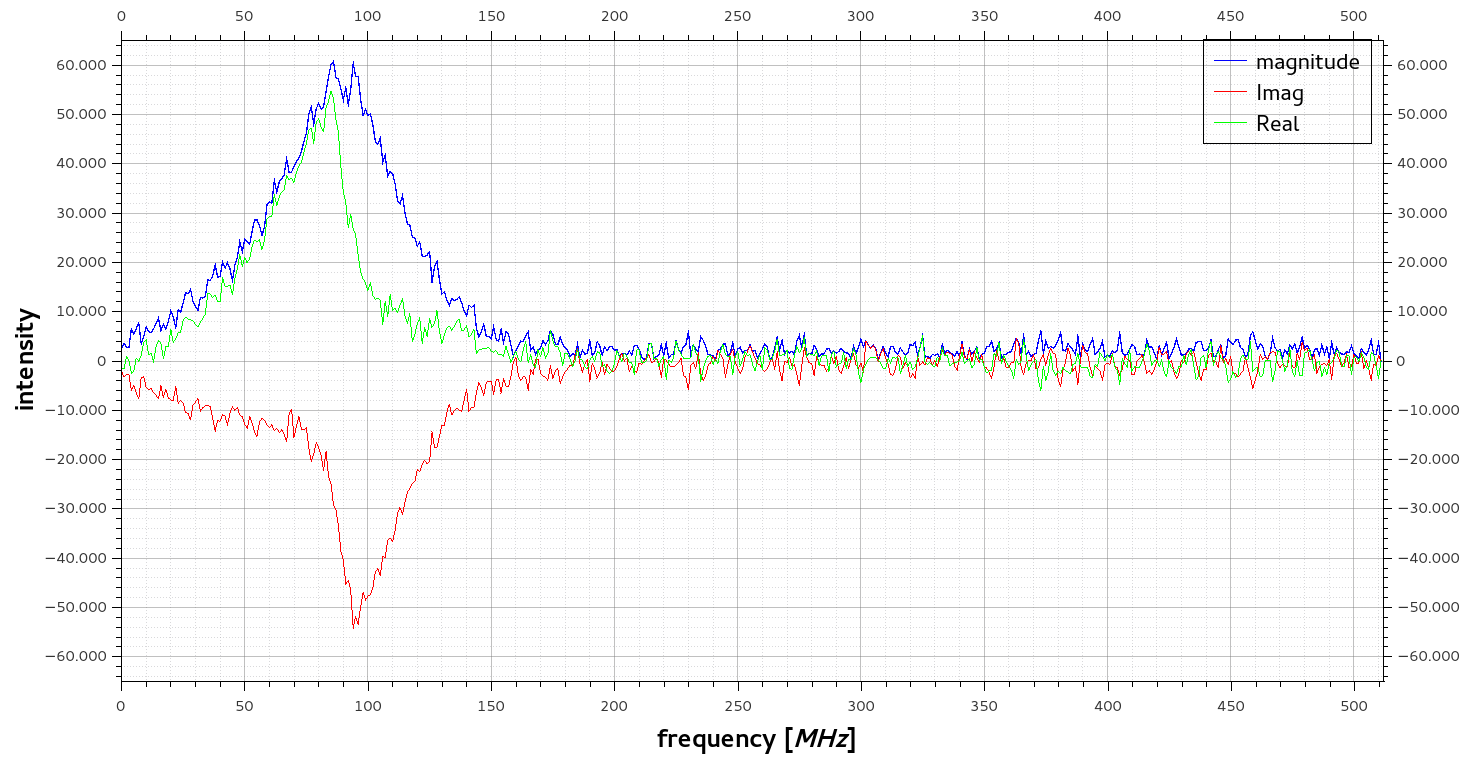
\includegraphics[scale=0.21]{pic/resfreq_td.png}}
            \subfigure[intensity at resonance frequency in fourier space\label{resfs}]{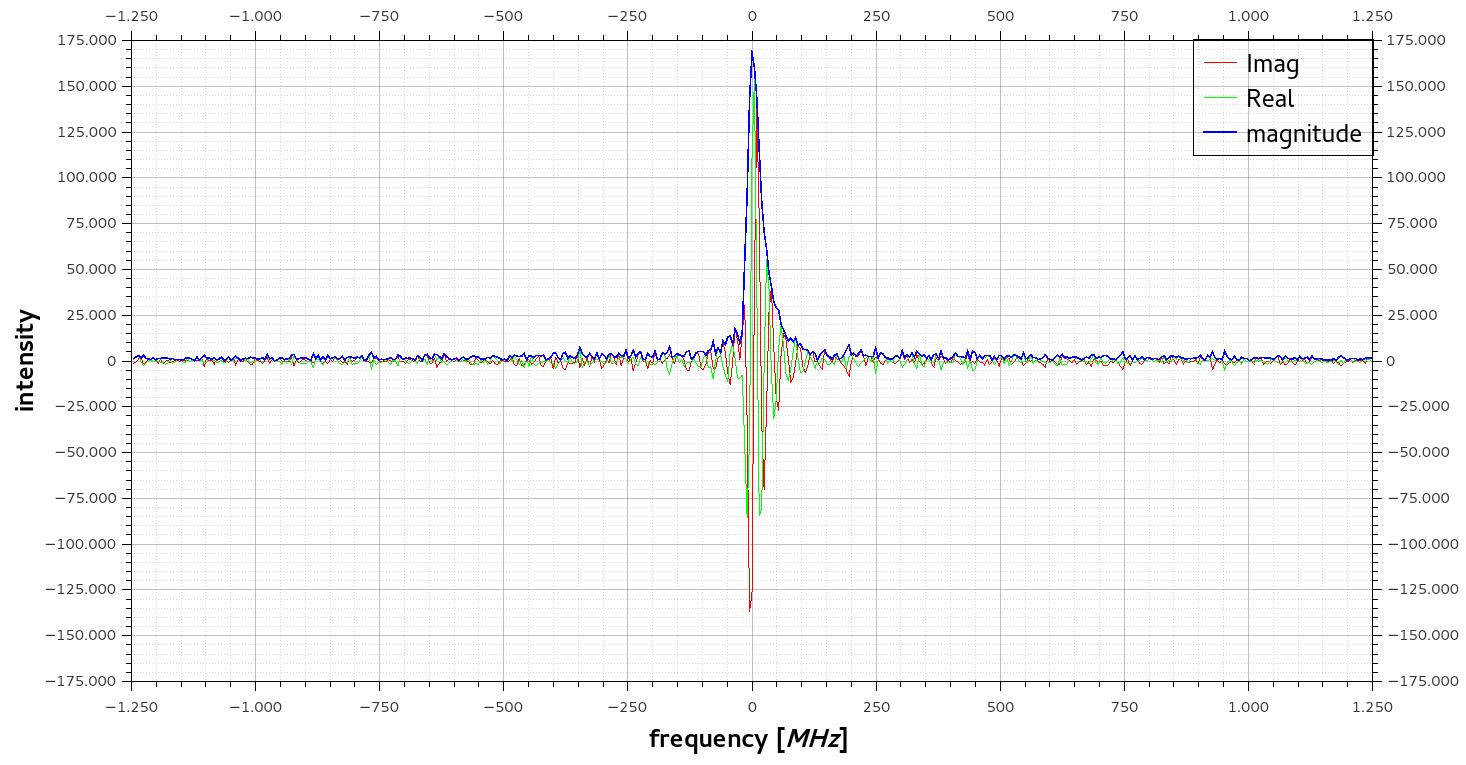
\includegraphics[scale=0.21]{pic/resfreq_fd.png}}
            \subfigure[intensity below resonance frequency in time domain\label{abotd}]{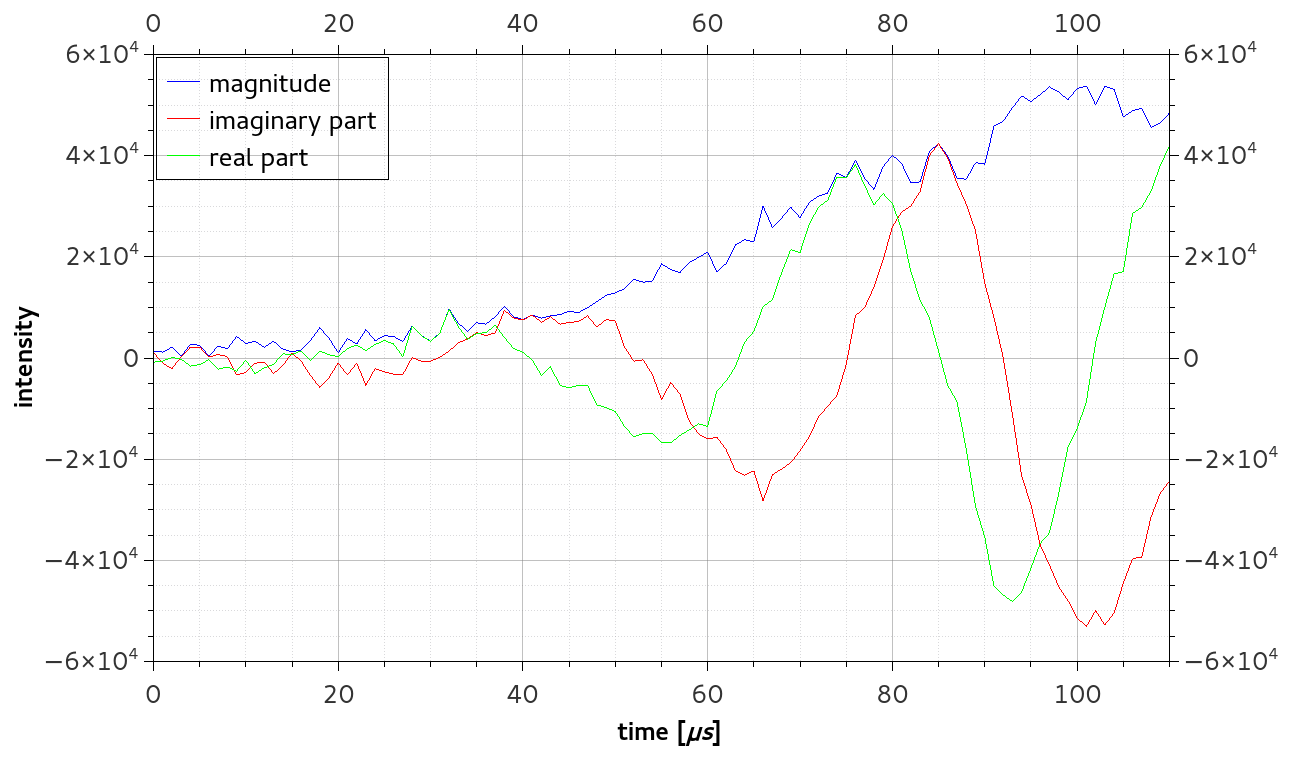
\includegraphics[scale=0.24]{pic/above_resfreq_td.png}}
            \subfigure[intensity below resonance frequency in fourier space\label{abofs}]{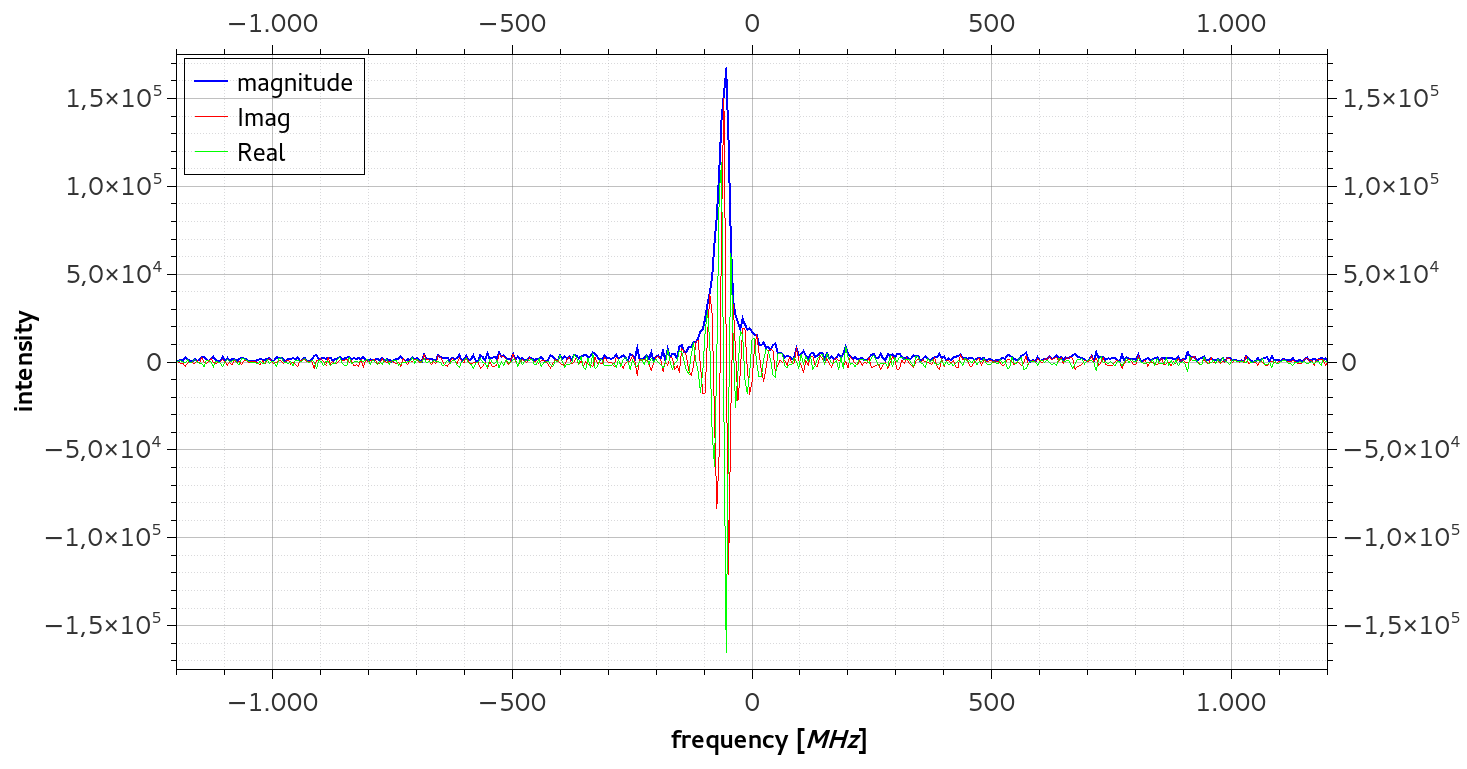
\includegraphics[scale=0.225]{pic/above_resfreq_fs.png}}
            \caption{Different spectra below, at and above the resonance frequency}
         \end{figure}
     One can see that the number of oscillations in \ref{abotd} and \ref{beltd} is bigger than in \ref{restd}. In figure \ref{resfs} one recognizes a good gaussian peak.
     With that information the frequency is found at $\omega_L = 45.47\unit{MHz}$. Using the $\gamma$-factor defined in (\ref{eq:gamma}) and the formula (\ref{eq:lamor}) one can calculate the magnetic field as $B_z = \omega_L/\gamma = 0.525\ \unit{T}$. This is a typical value for a magnetic flux density occuring in the bond of a solid state body.
         
    \subsection{Optimization of the pulse sequence by recording a rotation angle curve}
    \label{task_3}
    Now one can configure the time intevalls how long the measurement device should wait until it takes a measurement. In both cases, the spin-spin- and the spin-lattice-relaxation one get different times for $\tau$ aus one can see in the diagrams.
    After this measurements the computer takes all magnitude maxima as data points one can analyze.
           \begin{figure}[h]
               \centering
               \subfigure[another test\label{T2}]{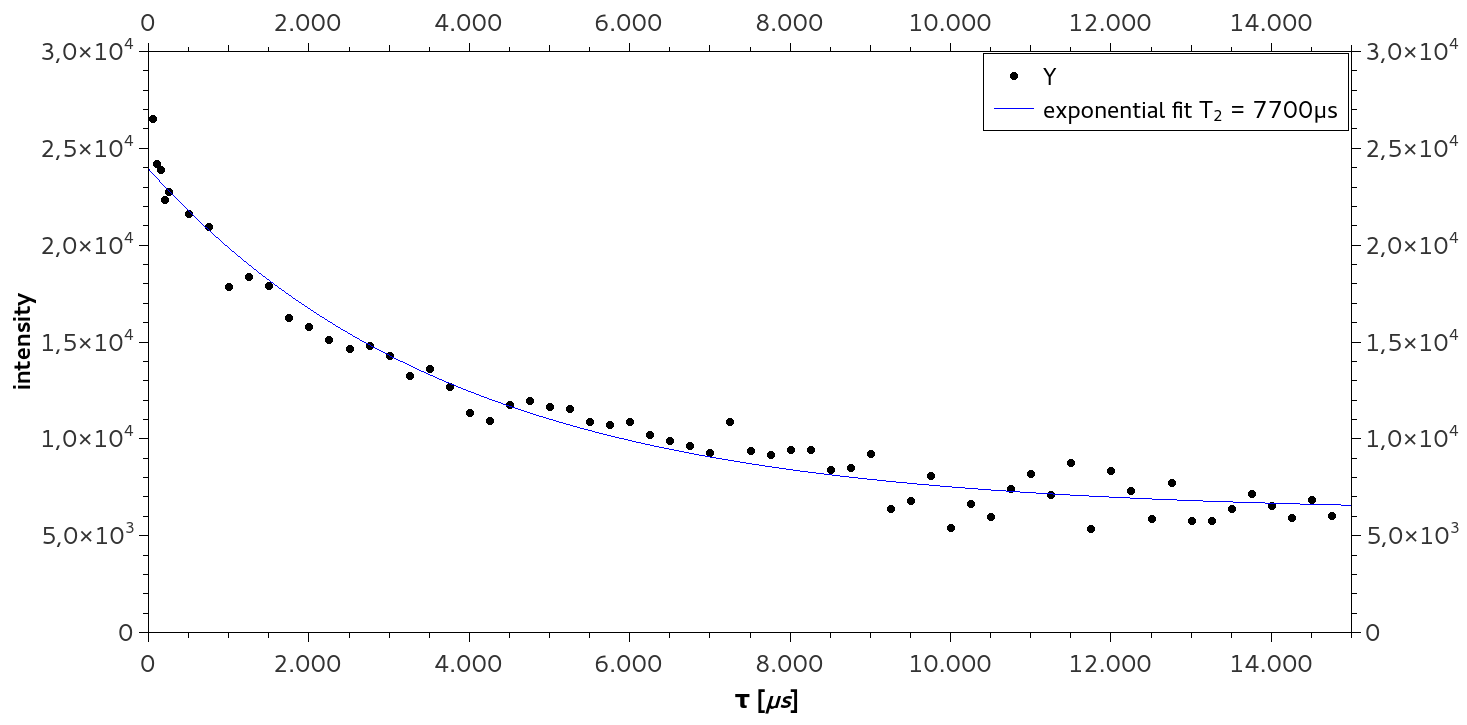
\includegraphics[scale=0.2]{pic/T2.png}}
               \subfigure[some test\label{T1}]{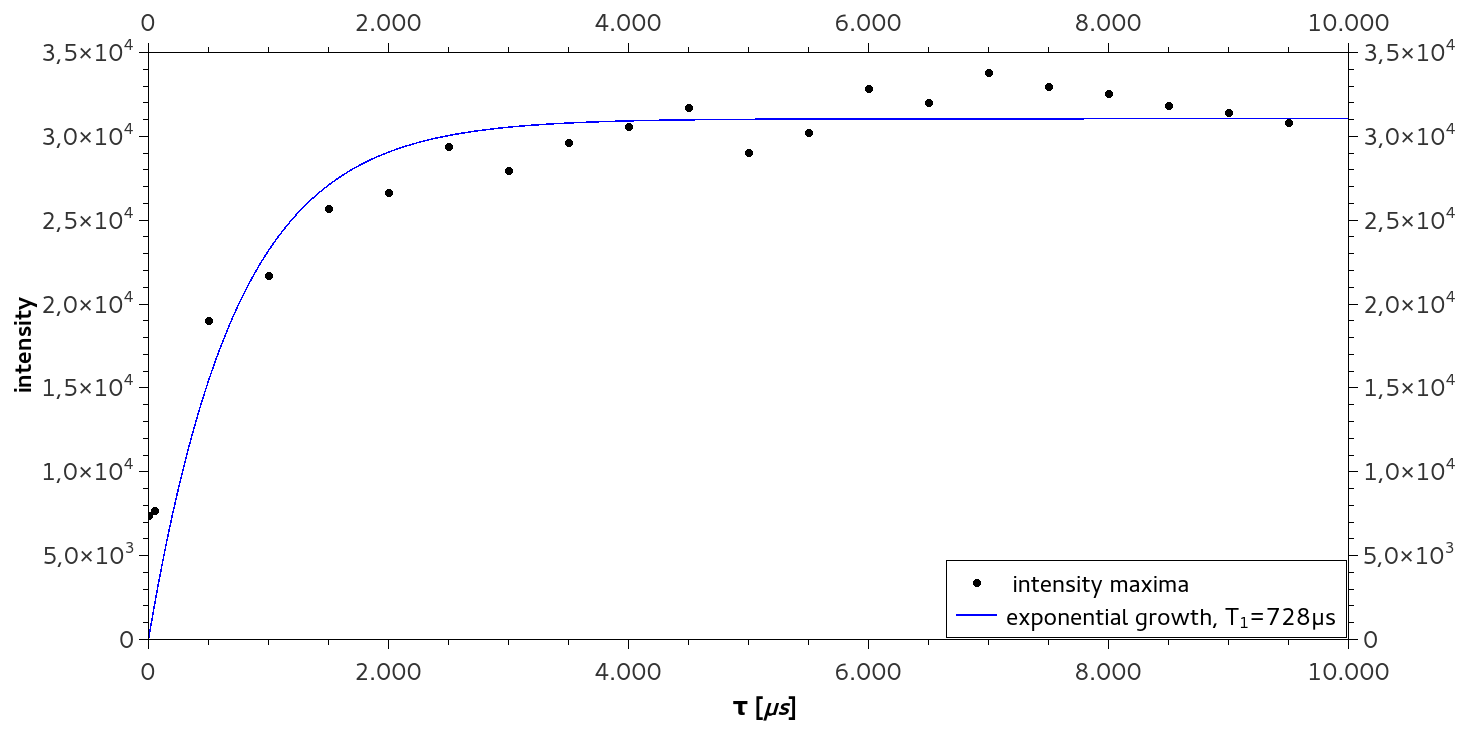
\includegraphics[scale=0.2]{pic/T1.png}}       
               \caption{rotation angle curves for spin-spin- (a) and spin-lattice-relaxation (b) }     
           \end{figure}
    One can recognize that \ref{T1} looks like an exponential growth and \ref{T2} looks similar to an exponential decay. To determine the relaxation constants one uses this information to make fits.        
    \subsection{Determination of the relaxation constants $T_1$ and $T_2$}
    The following fit functions are used;
    \begin{gather}
        y(\tau) = A\cdot(1-e^{-\tau/T_1})\label{fit_T1}\\
        y(\tau) = y_0 + Ae^{-2\tau/T_2}\label{fit_T2}
    \end{gather}
    With a tool called Qtiplot one makes a fit with these funktions a gets the blue line in \ref{T1} and \ref{T2}. The parameters for \ref{fit_T2} are: $A = 17720,\ y_0 = 6220$ and the spin-spin-relaxation constant $T_2 = 7628\unit{\mu s}$
    The parameters for the spin-lattice-relaxation are:
    $$ A = 31050,\ T_1 = 728\unit{\mu s} $$
    
    \label{task_4}
    In 
		% experimental procedure
\section{Data Analysis}

		% data analysis
\section{Discussion and conclusions}
	In the experiment the relaxation times $T_1$ and $T_2$ of an $^{57}$Fe spin ensemble were determined. The errors of the measurement are dominated by the deviation of the fits shown in the figures \ref{T1} and \ref{T2} that are because of the strong spreading relatively large. They could be reduced by taking several measurements for one constant value of the $\tau$ and $\Delta t$ time-variables. There also could be more abscissa-values for the fits all in all. The parameters one could choose in the measurement-software could also be improved.\\
	In the experiment we learned something about the behaviour of nuclear spins interacting with each other. The measured relaxation time-constants are strongly dependant on the environment where the spins are built-in such that the measurement of the relaxation-times provide the approach to investigate chemical bonds between atoms. In medical applications this fact is used to distinguish between tissues in Magnetic Resonance Tomography. There the nuclear spin of the hydrogen-atoms that are found in almost all organic molecules we are made of is used. Different organs and tissues consist of different organic structures so that the interaction of the hydrogen-spins with their environment is strongly depends on their location. Damadian showed in 1970 that relaxation-times of hydrongen within tumour-tissue are significantly larger than in their healthy counterparts. One reason for that is the increased water-ratio in the disseased tissue.\cite{t1Med} Table (\ref{t1_mrt}) shows this effect.\\
	\minipanf
	\centering
		\captionsetup{justification=raggedright, margin =4cm} 
		\begin{tabular}{c|cc}
			Tissue		&		$T_{1,h}$/s		&	$T_{1,t}$/s\\
			\hline
			skin		&		0.62			&	1.05\\
			lung		&		0.79			&	1.11\\
			bones		&		0.55			&	1.03\\
			stomach		&		0.76			&	1.23\\
			liver		&		0.57			&	0.83\\
		\end{tabular} 
		\captionof{table}{Dependancy of the $T_1$-relaxation time on different tissues. The index h stands for healthy tissue while t represents tumourous organs.\cite{t1Med}}
		\label{t1_mrt}
	\minipend
	\ \\
	These results can be tranferred to the considered iron-nuclei. If we would consider the atoms within a different chemical bond the relaxation times would differ from those we just measured. These investigations could be object of further experiments or theoretical models.
	

	% Auswertung bzw. Zusammenfassung
\begin{thebibliography}{99}
\bibitem [01] {PA} S. Diez. \textit{Advanced practical course - Experiment MMC}, Dresden, 2015
\bibitem [02] {t1Med} R. Winter, F.Noll. \textit{Methoden der Biophysikalischen Chemie}, Springer, 2013
\bibitem [03] {wikiKinesin} \texttt{https://en.wikipedia.org/wiki/Kinesin} [November 22, 2015]
\bibitem [04] {runLength} S. Ferbrugge et al. \textit{Novel ways to determine kinesin-1's run length and randomness using fluorescence microscopy}. Amsterdam. October 2009
\bibitem [05] {severalMP} S. Klumpp, R. Lipowsky.\textit{Cooperative cargo transport by several molecular motors}. Potsdam. November 2005
\end{thebibliography}

\end{document}